%================ Chapter ==================
\chapter{หลักการและทฤษฎีที่เกี่ยวข้อง}
\label{chap:theory}

%================ Section: Scrum Research ==================
\section{กระบวนการรวบรวมและเก็บข้อมูลตามหลัก Scrum}
\label{sec:scrum-research}

\noindent\textbf{วัตถุประสงค์} —
อธิบายแนวทางรวบรวมและตรวจสอบความต้องการภายใต้ Agile/Scrum เพื่อนำผลลัพธ์ไปใช้ต่อในการออกแบบและพัฒนาซอฟต์แวร์

\vspace{0.6em}
\noindent\textbf{ภาพรวมกระบวนการ}
\begin{enumerate}
  \item \textbf{แหล่งข้อมูล}: ใช้วิธีการต่างๆ เพื่อรวบรวมความต้องการ เช่น การสัมภาษณ์, การสังเกตการณ์ผู้ใช้, แบบสอบถาม และการวิเคราะห์ระบบเดิมหรือคู่แข่ง
  \item \textbf{สิ่งส่งมอบของ Scrum}: สร้างเอกสารหลักสำหรับการจัดการโครงการ ได้แก่ วิสัยทัศน์ผลิตภัณฑ์, รายการงานทั้งหมด, เรื่องราวของผู้ใช้, เกณฑ์การยอมรับงาน และข้อกำหนดว่าอะไรพร้อมทำงานหรืออะไรเสร็จสมบูรณ์แล้ว
  \item \textbf{รูปแบบ User Story}: เขียนความต้องการในมุมมองผู้ใช้ โดยใช้โครงสร้าง:
    \begin{quote}
      ในฐานะ \textit{[บทบาท]} \\
      ฉันต้องการ \textit{[ความสามารถ]} \\
      เพื่อที่จะ \textit{[ได้รับประโยชน์]}
    \end{quote}
  \item \textbf{การปรับแต่งแบ็กล็อก}: จัดการรายการงานโดยการจัดลำดับความสำคัญ, แบ่งงานใหญ่ให้เป็นงานย่อยที่จัดการได้ และเพิ่มรายละเอียดเงื่อนไขการยอมรับงาน
  \item \textbf{จังหวะการทำงาน}: ดำเนินงานเป็นวงจรซ้ำๆ เริ่มจากขั้นวางแผน 
    $\rightarrow$ พัฒนา $\rightarrow$ นำเสนอผลงาน $\rightarrow$ 
    เรียนรู้และปรับปรุง เพื่อพัฒนาความต้องการอย่างต่อเนื่อง
\end{enumerate}

\begin{figure}[h]
  \centering
  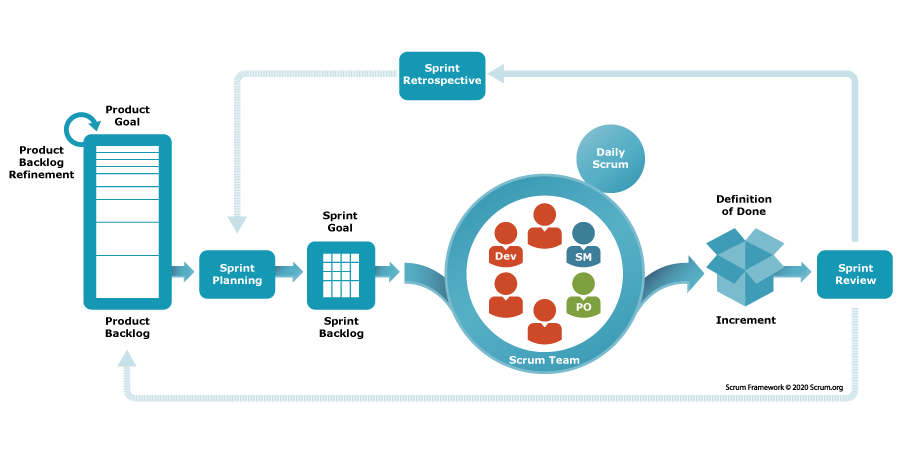
\includegraphics[width=.92\linewidth]{chapters/Images/SCRUM.png}
  \caption{แผนภาพแสดงหลักการพัฒนาซอฟต์แวร์แบบ Scrum}
  \label{fig:scrum-data-flow}
\end{figure}

%================ Section: DB Normalization & Index ==================
\section{หลักการออกแบบฐานข้อมูลโดยอิงตามหลัก Normal Form และ Index เพื่อประสิทธิภาพ}
\label{sec:db-normal-index}

\noindent
การออกแบบข้อมูลประกอบด้วยสองส่วนหลัก: \textbf{ความถูกต้องเชิงตรรกะ} (Normalization) และ \textbf{ประสิทธิภาพการเข้าถึง} (Indexing)

\subsection*{Normalization (1NF–3NF/BCNF)}
\begin{table}[h]
\centering
\begin{tabular}{@{}ll@{}}
\toprule
\textbf{นอร์มอลฟอร์ม} & \textbf{เกณฑ์หลักโดยย่อ} \\
\midrule
1NF & ค่าทุกช่องเป็นอะตอม ไม่มีกลุ่มซ้ำ/ซ้อน \\
2NF & อยู่ใน 1NF และไม่มีการพึ่งพาบางส่วนกับคีย์เชิงประกอบ \\
3NF & อยู่ใน 2NF และไม่มีการพึ่งพาแบบทรานซิทีฟกับคีย์ \\
BCNF & ทุกตัวกำหนด (determinant) ต้องเป็นคีย์แคนดิเดต \\
\bottomrule
\end{tabular}
\caption{สรุป Normal Forms ที่ใช้ในการออกแบบ}
\label{tab:nf}
\end{table}

\subsection*{Indexing เบื้องต้นเพื่อประสิทธิภาพ}
\begin{itemize}
  \item \textbf{ชนิดดัชนี}: B-tree (ทั่วไป/ช่วง), Hash (เท่ากับ), GiST/GIN (JSONB, full-text), BRIN (ตารางใหญ่เรียงตามช่วง)
  \item \textbf{หลักคิด}: เลือกคอลัมน์ที่มี selectivity สูง, ใช้ covering index กับคิวรีที่อ่านบ่อย, ระวังการทำดัชนีมากเกินไป (กระทบงานเขียน)
  \item \textbf{คอมโพสิตอินเด็กซ์}: จัดลำดับคอลัมน์ตาม WHERE/ORDER BY ที่พบบ่อย
\end{itemize}

\noindent\textit{ตัวอย่าง (แนวคิด)}:
\begin{verbatim}
-- คิวรีอ่านบ่อย: recent workouts ของผู้ใช้
CREATE INDEX idx_workout_user_time
ON workout(user_id, started_at DESC);

-- ค้นหา exercise ชื่อแบบ full-text (PostgreSQL)
CREATE INDEX idx_exercise_name_fts
ON exercise USING GIN (to_tsvector('simple', name));
\end{verbatim}

%================ Section: System Architecture ==================
\section{สถาปัตยกรรมของแอพนี้}
\label{sec:system-arch}

\noindent
สถาปัตยกรรมของระบบถูกออกแบบโดยผสมผสาน \textbf{Clean Architecture} สำหรับฝั่ง Backend และโครงสร้างมาตรฐานของ \textbf{Next.js/React Native} สำหรับฝั่ง Frontend เพื่อให้ได้ทั้งความเป็นระเบียบ ความสามารถในการขยาย และการบำรุงรักษาที่ง่ายในอนาคต

\subsection*{โครงสร้างโดยรวม}
\begin{itemize}
  \item \textbf{Client Layer}: 
    \begin{itemize}
      \item \textbf{Web Application} — พัฒนาโดย Next.js (React framework) ใช้โครงสร้างไฟล์มาตรฐาน \texttt{pages/}, \texttt{components/}, \texttt{api/}.
      \item \textbf{Mobile Application} — พัฒนาโดย React Native ตาม format ปกติ (โฟลเดอร์ \texttt{src/}, \texttt{screens/}, \texttt{navigation/}).
      \item รองรับ UI/UX ที่สอดคล้องกับ Figma prototype และมีการเชื่อมต่อ API ผ่าน RESTAPI
    \end{itemize}
  \item \textbf{Backend Layer (Clean Architecture)}:
    \begin{itemize}
      \item \textbf{Domain Layer} — กำหนด business rules, entity, และ interface ที่ไม่ขึ้นกับ framework
      \item \textbf{Use Case Layer} — ตรรกะการทำงาน เช่น การจัดการ workout plan, gamification badge, การวิเคราะห์ข้อมูล
      \item \textbf{Interface Adapter Layer} — แปลงข้อมูลระหว่าง use case/domain กับ external services (เช่น Database, API response)
      \item \textbf{Infrastructure Layer} — เชื่อมต่อกับ Database , Object Storage (ภาพ/วิดีโอ)
    \end{itemize}
  \item \textbf{Data Layer}: 
    \begin{itemize}
      \item ฐานข้อมูลเชิงธุรกรรม (PostgreSQL) สำหรับ core entities (user, workout, program, gamification)
      \item Object storage (เช่น MinIO) สำหรับไฟล์สื่อ เช่น รูป exercise และวิดีโอแนะนำ
    \end{itemize}
\end{itemize}

\subsection*{แนวคิดออกแบบสำคัญ}
\begin{itemize}
  \item \textbf{Separation of Concerns}: Frontend, Backend และ Data Layer ถูกแยกชัดเจน
  \item \textbf{Testability}: Clean Architecture ช่วยให้เขียน unit test ได้ง่าย เนื่องจาก business logic แยกออกจาก framework
  \item \textbf{Scalability}: รองรับการเพิ่มบริการใหม่ เช่น AI-based recommendation หรือ real-time tracking
  \item \textbf{Maintainability}: React/Next และ React Native ใช้ convention เดียวกับ community มาตรฐาน  $\rightarrow$  ลด learning curve สำหรับทีมใหม่
\end{itemize}


%================ Section: Security ==================
\section{หลักการรักษาข้อมูลที่ปลอดภัย}
\label{sec:security}

\noindent
ครอบคลุมความมั่นคงปลอดภัยข้อมูลและการคุ้มครองข้อมูลส่วนบุคคล (purpose limitation, data minimization, storage limitation) และการออกแบบ security by design

\begin{itemize}
  \item \textbf{การระบุตัวตน/การอนุญาต}: MFA, RBAC/ABAC, หลัก least privilege
  \item \textbf{การเข้ารหัส}: in transit (TLS), at rest (TDE/field-level), KMS
  \item \textbf{การเก็บรักษา}: นโยบายตามประเภทข้อมูล; pseudonymization/anonymization
  \item \textbf{การบันทึกเหตุการณ์}: Audit log, tamper-evident, breach notification
  \item \textbf{สิทธิของเจ้าของข้อมูล}: การเข้าถึง/แก้ไข/ลบ/จำกัด/พกพาข้อมูล
\end{itemize}

%================ Section: Health Science ==================
\section{วิทยาศาสตร์ทางด้านสุขภาพ}
\label{sec:health-science}

\noindent
วางรากฐานเชิงวิทยาศาสตร์สำหรับคุณลักษณะของระบบที่เกี่ยวกับการออกกำลังกายและพฤติกรรมผู้ใช้

\subsection{แนวทางของ ACSM (American College of Sports Medicine)}
\label{subsec:acsm}

\noindent
แนวทางจาก \textbf{ACSM} เป็นมาตรฐานสากลสำหรับการสั่งการออกกำลังกาย โดยอ้างอิงหลัก \textbf{FITT-VP} และขยายรายละเอียดสำหรับประชากรทั่วไป ดังนี้:

\begin{itemize}
  \item \textbf{แอโรบิก (Aerobic)}: อย่างน้อย 150 นาที/สัปดาห์ ของการออกกำลังกายระดับปานกลาง (หรือ 75 นาที/สัปดาห์ ของระดับหนัก) กระจาย 3–5 วัน/สัปดาห์
  \item \textbf{การฝึกแรงต้าน (Resistance Training)}: อย่างน้อย 2 วัน/สัปดาห์ ครอบคลุมกล้ามเนื้อหลักทุกมัด 8–12 ครั้ง/ท่า 2–4 เซ็ต
  \item \textbf{การยืดเหยียด (Flexibility)}: อย่างน้อย 2–3 วัน/สัปดาห์ ค้างแต่ละครั้ง 10–30 วินาที 2–4 รอบ
  \item \textbf{การฝึกประสาทและการเคลื่อนไหว (Neuromotor/Functional)}: อย่างน้อย 2–3 วัน/สัปดาห์ เช่น balance, agility, coordination, proprioception
  \item \textbf{หลักการเพิ่มเติม}: 
    \begin{itemize}
      \item ใช้ \%HRmax, \%HRR, RPE หรือ MET เป็นตัวกำหนดความหนัก
      \item ค่อยๆ เพิ่มภาระ (progressive overload) ตามสมรรถภาพและความปลอดภัย
      \item เน้นการออกกำลังกายที่หลากหลาย (multimodal) เพื่อลดการบาดเจ็บและเพิ่ม adherence
    \end{itemize}
\end{itemize}

